%% ----------------------------------------------------------------
%% Thesis.tex -- MAIN FILE (the one that you compile with LaTeX)
%% ---------------------------------------------------------------- 

% Set up the document
%\documentclass[a4paper, 12pt, twoside]{Thesis}  % Use the "Thesis" style, based on the ECS Thesis style by Steve Gunn
\documentclass[a4paper, oneside, 12pt]{Thesis}  % Use the "Thesis" style, based on the ECS Thesis style by Steve Gunn
\graphicspath{{Figures/}}  % Location of the graphics files (set up for graphics to be in PDF format)

% Include any extra LaTeX packages required
\usepackage[square, numbers, comma, sort&compress]{natbib}  % Use the "Natbib" style for the references in the Bibliography
\usepackage{verbatim}  % Needed for the "comment" environment to make LaTeX comments
\usepackage{vector}  % Allows "\bvec{}" and "\buvec{}" for "blackboard" style bold vectors in maths
\usepackage{float}
\hypersetup{urlcolor=blue, colorlinks=true}  % Colours hyperlinks in blue, but this can be distracting if there are many links.

%% ----------------------------------------------------------------
\begin{document}
\frontmatter	  % Begin Roman style (i, ii, iii, iv...) page numbering

% Set up the Title Page
\title  {HTML5 WebSocket protocol and its application to distributed computing}
\authors  {Gabriel Muller}
\addresses  {\groupname\\\DEPTNAME\\\univname\\\coursename}  % Do not change this here, instead these must be set in the "Thesis.cls" file, please look through it instead
\date       {\today}
\subject    {}
\keywords   {}

\maketitle
\makesecondtitle
%% ----------------------------------------------------------------

\setstretch{1.3}  % It is better to have smaller font and larger line spacing than the other way round

% Define the page headers using the FancyHdr package and set up for one-sided printing
\fancyhead{}  % Clears all page headers and footers
\rhead{\thepage}  % Sets the right side header to show the page number
\lhead{}  % Clears the left side page header

\pagestyle{fancy}  % Finally, use the "fancy" page style to implement the FancyHdr headers

%% ----------------------------------------------------------------
% Declaration Page required for the Thesis, your institution may give you a different text to place here
\Declaration{

I, Gabriel L. Muller, declare that this thesis titled, HTML5 WebSocket protocol and its application to distributed computing and the work presented in it are my own. I confirm that:

\begin{itemize} 
\item[\tiny{$\blacksquare$}] This work was done wholly or mainly while in candidature for a research degree at this University.
 
\item[\tiny{$\blacksquare$}] Where any part of this thesis has previously been submitted for a degree or any other qualification at this University or any other institution, this has been clearly stated.
 
\item[\tiny{$\blacksquare$}] Where I have consulted the published work of others, this is always clearly attributed.
 
\item[\tiny{$\blacksquare$}] Where I have quoted from the work of others, the source is always given. With the exception of such quotations, this thesis is entirely my own work.
 
\item[\tiny{$\blacksquare$}] I have acknowledged all main sources of help.
 
\item[\tiny{$\blacksquare$}] Where the thesis is based on work done by myself jointly with others, I have made clear exactly what was done by others and what I have contributed myself.
\\
\end{itemize}
 
 
%Signed:\\
%\rule[1em]{25em}{0.5pt}  % This prints a line for the signature
 
%Date:\\
%\rule[1em]{25em}{0.5pt}  % This prints a line to write the date


}
\clearpage  % Declaration ended, now start a new page

%% ----------------------------------------------------------------
% The "Funny Quote Page"
%\pagestyle{empty}  % No headers or footers for the following pages

%\null\vfill
% Now comes the "Funny Quote", written in italics
%\textit{``Write a funny quote here.''}

%\begin{flushright}
%If the quote is taken from someone, their name goes here
%\end{flushright}

%\vfill\vfill\vfill\vfill\vfill\vfill\null
%\clearpage  % Funny Quote page ended, start a new page
%% ----------------------------------------------------------------

% The Abstract Page
\chapter{Abstract}

%HTML5 WebSocket protocol brings real time communication in web browsers to a
new level. Daily, new products are designed to stay permanently connected to
the web. WebSocket is the technology enabling this revolution. WebSockets are
supported by all current browsers, but it is still a new technology in constant
evolution.

WebSockets are slowly replacing older client-server communication
technologies. As opposed to comet-like technologies WebSockets' remarkable
performances is a result of the protocol's fully duplex nature and because it
doesn't rely on HTTP communications.

To begin with this paper studies the WebSocket protocol and different 
WebSocket servers implementations. This first theoretic part focuses more 
deeply on heterogeneous implementations and OpenCL. The second part is
a benchmark of a new promising library. 

The real-time engine used for testing purposes is SocketCluster. SocketCluster
provides a highly scalable WebSocket server that makes use of all available cpu
cores on an instance. The scope of this work is reduced to vertical scaling of 
SocketCluster.




The Thesis Abstract is written here (and usually kept to just this page). The page is kept centered vertically so can expand into the blank space above the title too\ldots


\clearpage  % Abstract ended, start a new page
%% ----------------------------------------------------------------

\setstretch{1.3}  % Reset the line-spacing to 1.3 for body text (if it has changed)

% The Acknowledgements page, for thanking everyone
\chapter{Acknowledgements}

\chapter*{Acknowledgements}
 


\clearpage  % End of the Acknowledgements
%% ----------------------------------------------------------------

\pagestyle{fancy}  %The page style headers have been "empty" all this time, now use the "fancy" headers as defined before to bring them back


%% ----------------------------------------------------------------
\lhead{\emph{Contents}}  % Set the left side page header to "Contents"
\tableofcontents  % Write out the Table of Contents

%% ----------------------------------------------------------------
\lhead{\emph{List of Figures}}  % Set the left side page header to "List if Figures"
%\listoffigures  % Write out the List of Figures

%% ----------------------------------------------------------------
\lhead{\emph{List of Tables}}  % Set the left side page header to "List of Tables"
\listoftables  % Write out the List of Tables

%% ----------------------------------------------------------------
\setstretch{1.5}  % Set the line spacing to 1.5, this makes the following tables easier to read
\clearpage  % Start a new page
\lhead{\emph{Abbreviations}}  % Set the left side page header to "Abbreviations"
\listofsymbols{ll}  % Include a list of Abbreviations (a table of two columns)
{
% \textbf{Acronym} & \textbf{W}hat (it) \textbf{S}tands \textbf{F}or \\
\textbf{LAH} & \textbf{L}ist \textbf{A}bbreviations \textbf{H}ere \\

}

%% ----------------------------------------------------------------
% End of the pre-able, contents and lists of things
% Begin the Dedication page

\setstretch{1.3}  % Return the line spacing back to 1.3

\pagestyle{empty}  % Page style needs to be empty for this page
%\dedicatory{For/Dedicated to/To my\ldots}

\addtocontents{toc}{\vspace{2em}}  % Add a gap in the Contents, for aesthetics


%% ----------------------------------------------------------------
\mainmatter	  % Begin normal, numeric (1,2,3...) page numbering
\pagestyle{fancy}  % Return the page headers back to the "fancy" style

% Include the chapters of the thesis, as separate files
% Just uncomment the lines as you write the chapters

\chapter{Introduction} 
\label{Chapter1}
\lhead{Chapter 1. \emph{Introduction}}

This first chapter ..\\

\section{Javascript}

In order to keep up with the evolution and continuous growth of the Internet, web technologies have been undergoing significant upgrades. Since 2007, the World Wide Web Consortium (W3C) has been working on a major update of the core language of the web that renders and displays all web contents. This is known as the 5th revision of Hyper Text Markup Language (HTML5). 
However the slow performance of JavaScript in performing dynamic operations is a serious limiting factor to wider use.  Improving the efficiency of JavaScript is an active field of research.\\

\section{Client server communications}

Client – server communication have been built around the HTTP protocol. CHANGE INTRO ..\\

\subsection{HTTP protocol}

The HTTP protocol is a request/response protocol. A client sends a request to the server in the form of a request method, URI, and protocol version, followed by a MIME-like message containing request modifiers, client information, and possible body content over a connection with a server. The server responds with a status line, including the message's protocol version and a success or error code, followed by a MIME-like message containing server information, entity meta information, and possible entity-body content. \citep{Reference1}\\

Because HTTP was not designed for real time communication several workarounds have been developped over the years to over come the so called page by page model. These techniques are nicely resumed in Eliot Step master thesis \citep{Reference2}.

\subsection{Page by page model}

Since HTTP's release in 1991, client server communication have undergone continuous upgrades. In the early twenties, most web pages were static. As a consequence, the client server communication were rather limited. Typically, the client would send from time to time a request to the server, the server would then answer back. All communication would then stop until the client triggered a new event.\\

\begin{figure}[htbp]
	\centering
		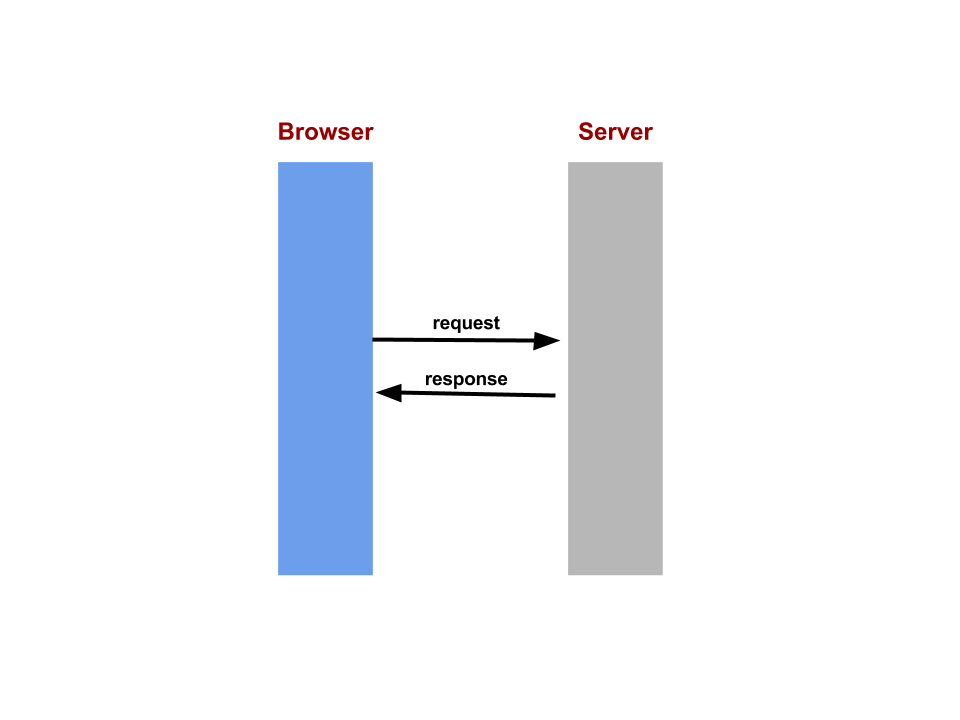
\includegraphics[width=0.9\textwidth]{./Figures/client_server_communication.png}
	\caption[client_server_communication]{Client server communication}
	\label{fig:client_server_communication}
\end{figure}

The notion of dynamic web appeared in 2005 with the apparition of technologies like Comet. Peter Lubbers describes it as the Headache 2.0 in his article \textit{A quantum leap in scalability for the web} \citep{Reference32}.\\

\subsection{1.2.3 – Polling}

Polling was the first attempt for real-time communication. Instead of waiting for the client to manually ask for a page update, the browser was sends regular HTTP GET requests to the server. This technique could be efficient if the exact interval of update on the server side was known.\\

However real time information are unpredictable and in high updates rate situation like for example stock prices, news reports or tickets sales the response could be stale by the time the browser renders the page \citep{Reference32}.\\
Also in low updates rate situation even if no data is available, the server will send an empty response. Resulting in a large amount of unnecessary connections beeing established which over time and with the clients increase leads to decreased overall network throughput \citep{Reference2}. \\

\begin{figure}[htbp]
	\centering
		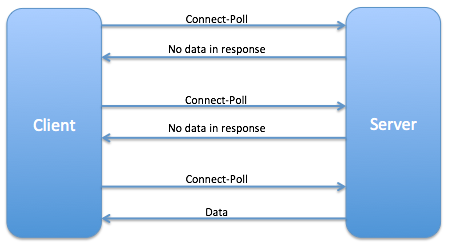
\includegraphics[width=0.9\textwidth]{./Figures/polling.png}
	\caption[polling]{polling}
	\label{fig:polling}
\end{figure}

\subsection{Long polling}

Long polling is based on Comet technologies and is slight step further toward server events and real time communication. Comet began to be popular in web browser around 2007, it is a family of web techniques that allows the server to hold an HTTP request open for prolonged periods of time.\\

Long-polling is similar to polling, except that the server keeps the HTTP request open if data is not immediately available. The server determines how long to keep the request open, also known as a hanging GET". If new data is received within the time interval, a response containing the data is sent to the client and the connection is closed. If new data is not received within the time period, the server will respond with a notification to terminate the open request and close the connection. After the client browser receives the response, it will create another XHR object request to handle the next event, therefore always keeping a new long-polling request open for new events. This results in the server constantly responding with new data as soon as it is made available \citep{Reference2}.\\

However, in situations with high-message volume, long- polling does not provide increased performance benefits over regular polling. Performance could actually be decreased if long-polling requests turn into continuous, unthrottled loops of regular polling requests.\\

\begin{figure}[htbp]
	\centering
		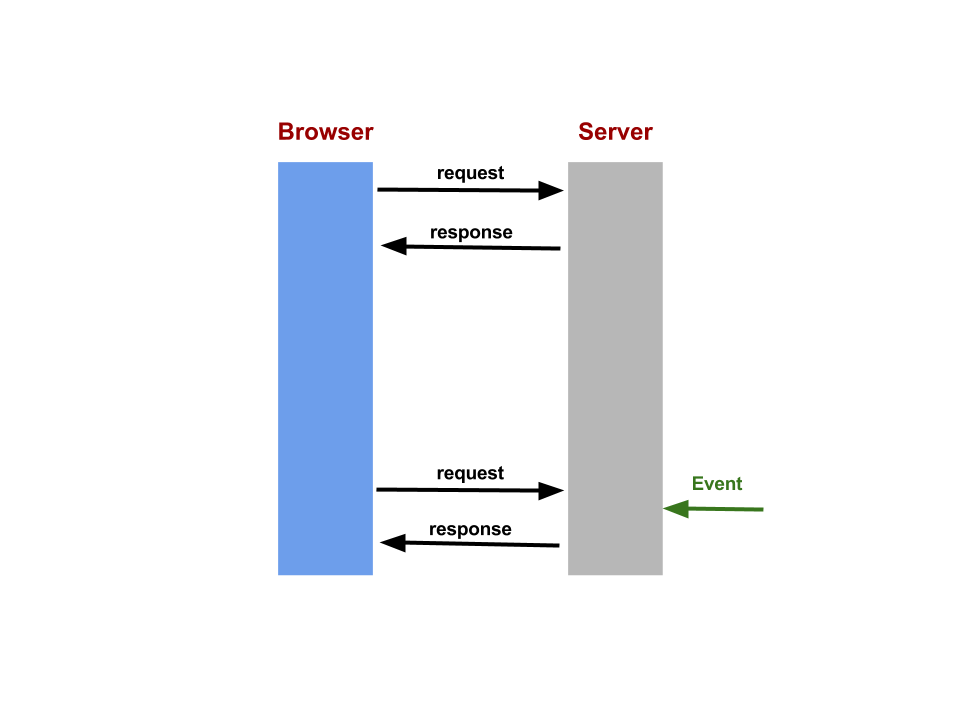
\includegraphics[width=0.9\textwidth]{./Figures/long_polling.png}
	\caption[long_polling]{Long polling}
	\label{fig:long_polling}
\end{figure}
	
\subsection{Streaming}

Streaming is based on a persistent HTTP connection. The communication still begins with a request from the browser, the difference is in the response. The server never signals the browser its message is finished. This way the connection is kept open and ready to deliver futher data. \citep{Reference2}.\\

Wouldn't it be because of proxies, streaming would be a perfectly adapted for real time communication. Because streaming is done over HTTP,  proxy server may choose to buffer server responses and thus increasing greatly the latency of the message delivery. Therefore in case a proxy is detected most Comet-like solution fall back to long polling \citep{Reference2}.\\

\begin{figure}[htbp]
	\centering
		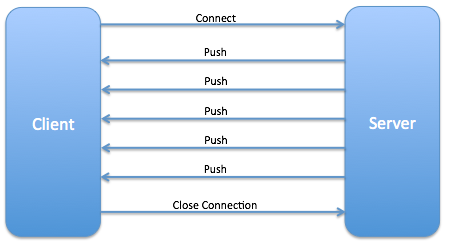
\includegraphics[width=0.9\textwidth]{./Figures/streaming.png}
	\caption[streaming]{Streaming}
	\label{fig:streaming}
\end{figure}

\subsection{Current technologies in browser}

At the moment, comet technologies are still the most popular way of communication between browsers and servers. The technique has been improved to the point where it perfectly fakes server sent event. Comet technologies can be seen as a wonderful hack to reach real time communication. However little can be done to improve the latency. Comet technologies resolve around HTTP and carry its overhead\\

The total overhead from the HTTP request and response header is at least 871 bytes without containing any data. In comparaison, a small payload is 20 bytes. Contempory application like on-line games can not be built on a technology waisting ressources equivalent to 40 messages every time informations are exchanged \citep{Reference2}. Therefore a brand new protocol has been developed: WebSocket.\\

\section{WebSocket protocol}

The creation of the WebSocket protocol marks the begenning of the Living web. It is often referred to as the first major upgrade in the history of web communications. As the Web itself originally did, WebSocket enables entirely new kinds of applications. Daily, new products are designed to stay permanently connected to the web. Websocket is the language enabling this revolution.\\

The official Request For Comments \citep{Reference12} (RFC) describes the WebSocket protocol as follows.\\

The WebSocket Protocol enables two-way communication between a client running untrusted code in a controlled environment to a remote host that has opted-in to communications from that code.  The security model used for this is the origin-based security model commonly used by web browsers.  The protocol consists of an opening handshake followed by basic message framing, layered over TCP.  The goal of this technology is to provide a mechanism for browser-based applications that need two-way communication with servers that does not rely on opening multiple HTTP connections.\\

This section is structured to follow step by step the creation of a WebSocket communication channel. The first subsection is about the initialization of this channel also called handshake. The second about the transport layer. After what the messages frame anatomy will be discussed and to finish WebSocket's behavior toward firewalls will be briefly described.\\

\subsection{The WebSocket handshake}

The Websocket protocol was to be released in an already existing web infrastrucure. Therefore it has been designed to be backward-compatible. Before a Websocket communication can start, a HTTP connection must be initiated. The browser sends an Upgrade header to the server to inform him he wants to start a WebSocket connection. Switching from the HTTP protocol to the WebSocket protocol is referred to as a handshake \citep{Reference12}.\\ 

\begin{verbatim}
GET ws://websocket.example.com/ HTTP/1.1
Origin: http://example.com
Connection: Upgrade
Host: websocket.example.com
Upgrade: websocket
\end{verbatim}

If the server supports the WebSocket protocol, it sends the following header in response.\\

\begin{verbatim}
HTTP/1.1 101 WebSocket Protocol Handshake
Date: Wed, 5 May 2014 04:04:22 GMT
Connection: Upgrade
Upgrade: WebSocket
\end{verbatim}

After the completion of the handshake the WebSocket connection is active and either the client or the server can send data. The data is contained in frames, each frame is prefixed with a 4-12 bytes to ensure the message can be reconstructed. \\
Once the server and the browser have agreed on begenning a WebSocket communication. A first request is made to begin an ethernet communication followed by a request to make an TCP / IP communication.\\

\subsection{Transport layer protocol }

The internet is based on two transport layer protocol, the User Datagram Protocol (UDP) and the Transmission Control Protocol (TCP). Both use the network layer service provided by the internet protocol (IP). \\

\textbf{TCP}

TCP is a reliable transmission protocol. The data is buffered bytes by bytes in segments and transmitted according to specific timers. This flow control ensures the consistancy of the data. TCP is said to be a stream oriented because the data is sent in independent segments.\\

\textbf{UDP}

UDP is an unreliable but fast transmission protocol. The protocol offers no guarentees the data will be delivered in its integrality nor duplicated. It works on a best effort strategy with no flow control. Each segments are received independently, it is a message oriented protocol.\\

Websocket is build over TCP because of its realiability. Browser enabled games are the perfect use case example of WebSockets. They require low latency even though the rate of update is rather high. To achieve a low latency, the communication protocol must make sure not to drop any packets. Otherwise, the exhange takes two times longer.\\
As can be inferred from the 2 previous subsections, the websockets protocol is depedant of quite a few other protocols. Namely HTTP to initialize the communication then ethernet, TCP/IP and finaly  TLS in case a secure connections is required. The next subsections looks more in details the anatomy of the frames sends over the web when using the websocket protocol.\\

\subsection{The WebSocket frame anatomy}

The study conducted by Tobias Oberstein \citep{Reference30} looks into the overheads of websockets. As a matter of fact the overhead induced purely by WebSockets is extremely low. As can be seen in the figure \ref{fig:frame_overhead}, depending on the size of the payload the overhead varies between 8 and 20 bytes.\\

\begin{figure}[htbp]
	\centering
		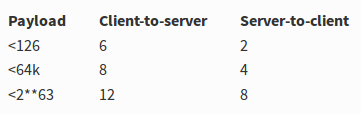
\includegraphics[width=0.5\textwidth]{./Figures/frame_overhead.png}
	\caption[frame_overhead]{Frame overhead \citep{Reference30}}
	\label{fig:frame_overhead}
\end{figure}


However, as pointed out in the article efficiency is lost on all other layers the websocket protocol relies on. Figure \ref{fig:tls_overhead} and \ref{fig:tcp_overhead} show respectively the overhead induced by pure tcp/ip and tls protocols.\\

\begin{figure}[htbp]
	\centering
		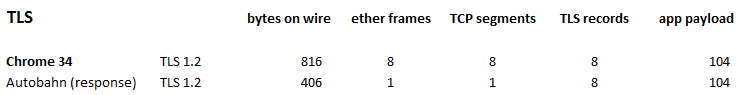
\includegraphics[width=0.9\textwidth]{./Figures/tls_overhead.png}
	\caption[tls_overhead]{TLS overhead \citep{Reference30}}
	\label{fig:tls_overhead}
\end{figure}

\begin{figure}[htbp]
	\centering
		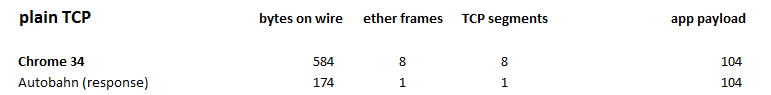
\includegraphics[width=0.9\textwidth]{./Figures/tcp_overhead.png}
	\caption[tcp_overhead]{TCP overhead \citep{Reference30}}
	\label{fig:tcp_overhead}
\end{figure}



In this example, the payloads \textit{Hello world”} is only therteen bytes. In comparaison, the ethernet, tcp/ip and tls protocols each use height bytes. The conclusion of this article is to warn programmers about the size of the payloads to make sure ethernet, tcp/ip and tls protocols don't dwarf the overhead of WebSocket itself. 
In case small payloads can not be avoided a possible solution is to serialize the messages in order to  batch them in one single WebSocket message.\\

So instead of sending the each messages using the WebSocket protocol like it is done in figure x. The individual messages are put in a queue and batched in a single Websocket message like in figure y.


\begin{figure}[htbp]
	\centering
		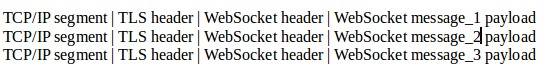
\includegraphics[width=0.7\textwidth]{./Figures/separate_websocket.png}
	\caption[separate_websocket]{WebSocket messages sent individualy \citep{Reference30}}
	\label{fig:separate_websocket}
\end{figure}

\begin{figure}[htbp]
	\centering
		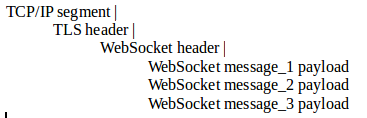
\includegraphics[width=0.5\textwidth]{./Figures/batched_websocket.png}
	\caption[batched_websocket]{Batched WebSocket messages \citep{Reference30}}
	\label{fig:batched_websocket}
\end{figure}

Never the less, WebSockets carry way less overheads then comet technologies does. Another advantage of WebSocket its interaction with proxies.\\

\subsection{Proxies}

Proxy servers are set up between a private network and the Internet. They act like an intermediary providing content caching, security and content filtering.\\

When a Websocket server detects the presence of a proxy server, it automatically sets up a tunnel to pass through the proxy. The tunnel is established by issuing an HTTP CONNECT statement to the proxy server, which requests for the proxy server to open a TCP/IP connection to a specific host and port. Once the tunnel is set up, communication can flow unimpeded through the proxy.\\

LINK

\section{Scope of the thesis}
\section{Thesis structure}
 % Introduction

\chapter{Literrature review} 
\label{Chapter2} 
\lhead{Chapter 2.\emph{Literrature review}}

This second chapter studies research done around WebSockets. The first
section is about the implementation of WebSockets server, the second is about
scalability. \\

\section{Implementation}

As in any project, in order to avoid future technical problems, it is better to
first study similar projects. The goal of this implementation study is to find a
suitable language and possibly a good library to run the experiment.

\subsection{WebSocket server implementation}

In order to narrow the library study, first a language needs to be selected.

\textbf{Language Selection}

Choosing a language for a project is often a compromise between the programmer
development background and the necessity of the application. Furthermore,
WebSocket servers can be developped in almost any languages.\\

This subsection does not aim at giving a comprehensive comparaison of all
existing WebSocket friendly languages. Node.js seems to be the perfect
environment for this study, therefore other languages will deliberatly be left
apart and the focus will be on explaining why Node.js is appropriate.\\

Node.js was specially invented to create real-time websites with push
capabilities \citep{Reference35}. Most languages run parallel tasks by using
threads but threads are memory expensive. Node.js is fundamentally different,
it runs as a single non-blocking and event-driven loop by using asynchronous
call back loops \citep{Reference37}. For this reasons, compared to other
languages, Node.js performs significantly better in highly concurrent
environment.\\

Node.js has many real-time engines. The next step is to carefully make a choice
between ws, Socket.io and Engine.io.\\  

\textbf{WebSocket implementation selection}

Deniz Ozger article's for medium.com \citep{Reference36} is a comprehensive study
of node.js real-time engines.\\

Ws is a pure WebSocket implementation, therefore it is interesting for testing
purpose but seldom used in real life projects.  The main drawback is the
communication may not work in case the browser does not support WebSockets.\\

Socket.io has some appreciable features namely it's connection procedure. First
it tries to connect to a server via WebSocket, in case it fails it downgrades
until it founds a suitable protocol. Moreover it tries to reconnect sockets
when connections fail.\\ 

Engine.io is a lower library of Socket.io. The connection procedure is the
opposite to Socket.io though. It first establishes a long polling connection
and only later tries to upgrade it to a better transport protocol. Therefore it
is more reliable because it establishes less connection.\\

In conclusion, Node.js and its real-time library engine.io seems a good choice
for our experiment. However better perfomance could be reached using an
heterogeneous implementation.


\subsection{Heterogeneous implementation with OpenCL}

As suggest John Stone paper's title \texttt{OpenCL: A parallel programming standard
for heterogeneous computing systems} \citep{Reference5} OpenCL is unanimously
considered as the refetence for heterogenous computing.\\

Historically, the first technology to take advantage of the massive parallel
nature of GPUs was Open Graphic Library (OpenGL). OpenGL is an application
programming interface (API) for rendering 2D and 3D vector graphics. Through
the insertion of little pieces of C-like codes in shader, developpers soon
realized graphic processing units (GPUs) could also be used for general
programming. This became known as General Purpose computation on GPUs (GPGPU)
\citep{Reference5}.\\

However, shadders can only be modified so much. As the need for more complex
applications arose Apple proposed the Khronos Group to develop a more general
framework: OpenCL. OpenCL is a low-level API accelerating applications with
task-parallel or data-parallel computations in a heterogeneous computing
environment. Indeed OpenCL not only allows the usage of CPUs but also any
processing devices like GPUs, DSPs, accelerators and so on \citep{Reference5}.
If generally on desktop the diversity of processing devices is quite low, it is
the opposite for mobile. Embedded systems for real-time multimedia journal
published a paper \citep{Reference3} highlining the advantages of using OpenCl
in mobile browser.\\

OpenCL doesn't guarantee a particular kernel will achieve peak performance on
different architectures. The nature of the underlying hardware may induce
different programming strategies. Multi-core CPU architecture is definitely the
more popular. But the recent specification published by Khronos to take GPU
computing to the web is bound to raise programmers interest toward GPUs
architecture \citep{Reference30}.\\ 

\textbf{CPUs architecture}

Modern CPUs are typically composed of a few high-frequency processor cores.
CPUs perform well for a wide variety of applications, but they are optimal for
latency sensitive workloads with minimal parallelism. However, to increase
performance during arithmetic and multimedia workloads,  many CPUs also
incorporate small scale use of single instruction multiple data (SIMD).\\

\textbf{GPUs architecture}

Contemporary GPUs are composed of hundreds of processing units running at low
frequency. \\

As a result GPUs are able to execute tens of thousands of threads. It is this
ability which makes them so much more effective then CPUs in a highly parallel
environment. Some research even claim a speedup in the order of 200x over
JavaScript. \citep{Reference3}\\

The GPU processing units are typically organized in SIMD clusters controlled by
single instruction decoders, with shared access to fast on-chip caches and
shared memories. Massively parallel arithmetic-heavy hardware design enables
GPUs to achieve single-precision floating point arithmetic rates approaching 2
trillions of instructions per second (TFLOPS). \citep{Reference5}\\

Although GPUs are powerful computing devices, currently they still often
require to be managemed by a host CPU. Fortunately OpenCL is designed to be used in
heterogeneous environment. It abstracts CPUs and GPUs as “compute devices”.
This way, applications can query device attributes to determine the
properties of the available compute units and memory systems.
\citep{Reference5}\\

All the same, even if OpenCL's API hides the hardest part of parallel
programming a good understanding of the underlying memory model leads to more
efficient codding. Along with general advises on how to build an OpenCL
cluster, details about the memory model are given in the following paper:
\citep{Reference4}.\\

\textbf{Platform model}

CPU and GPU are called “compute devices”. A single host regroups one or more
compute devices and has its own memory. Each compute device is composed of one
or more cores also called “compute units”. Each compute unit has its own memory
and is divided into one or more SIMD threads or “processing elements” with its
own memory. \citep{Reference4}\\

\begin{figure}[H] \centering
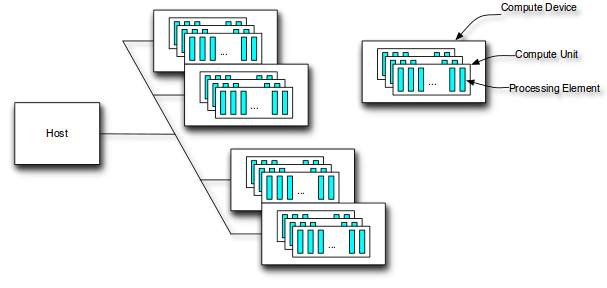
\includegraphics[width=\textwidth]{./Figures/plateform_model.png}
\caption[Plateform model]{Plateform model \citep{Reference4}}
\label{fig:plateform_model} \end{figure}


\textbf{Memory model}

OpenCL defines 4 types of memory spaces within a compute device. A large
high-latency “global” memory corresponding to the device RAM. This is a none
cached memory  where the data is stored and is available to all items. A small
low-latency read-only “constant” memory which is cached. A shared “local”
memory accessible from multiple processing elements within the same compute
unit and a “private” memory accessible within each processing element. This
last type of memory is very fast and is the register of the items
\citep{Reference4}.\\

\begin{figure}[H] \centering
  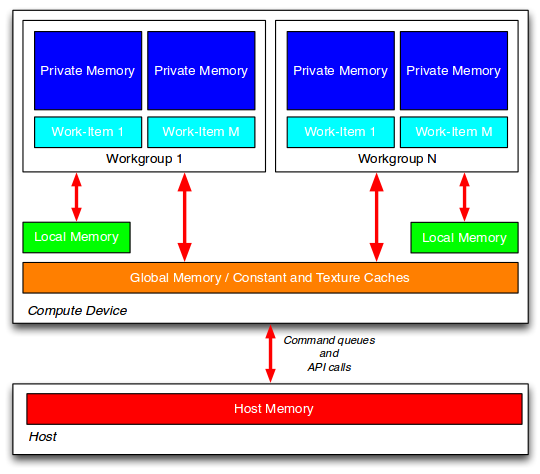
\includegraphics[width=0.6\textwidth]{./Figures/memory_model.png}
  \caption[Memory model]{Memory model \citep{Reference4}}
  \label{fig:memory_model} 
\end{figure}

In conclusion, OpenCL provides a fairly easy way to write parallel code but to
reach an optimal performance / memory access trade off programmers must choose
carefully in where to save their variables in memory space.\\

\textbf{Global and local IDs}

Finally, at an even lower level, work-items are scheduled in work–groups.
This is the smallest unit of parallelism on a device. Individual work-items in
a work–group  start together at the same program address, but they have their
own address counter and register state and are therefore free to branch and
execute independently \citep{Reference4}.\\

\begin{figure}[H] \centering
  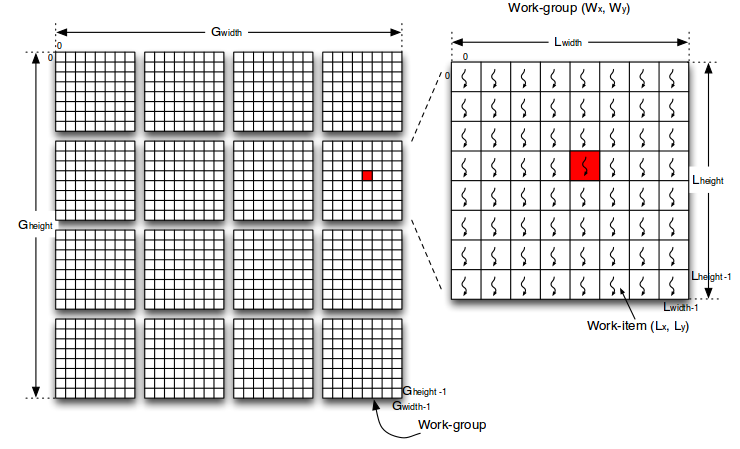
\includegraphics[width=\textwidth]{./Figures/id.png} 
  \caption[Work - group]{Work Group \citep{Reference4}} 
  \label{fig:id} 
\end{figure}


On a CPU, operating systems often swap two threads on and off execution
channels. Threads (cores ) are generally heavyweight entities and those context
switches are therefore expensive. By comparison, threads on a GPU ( work-items
) are extremely lightweight entities. Furthermore in GPUs, registers are
allocated to active threads only. Once threads are complete, its resources are
de-allocated.  Thus no swapping of registers or state occurs between GPU
threads. \citep{Reference4}\\

As can be deduced from this section about the underlying memory model, OpenCL is a
fairly low-level API. In fact, the programming language used is a derivate of
the C language based on C99. A language web developers will most likely be
unfamiliar with. Khronos anticipated this and developed the web computing
language (WebCL).\\

\subsection{WebCL}

WebGL and WebCL are JavaScript APIs over OpenGL and OpenCL's API. This allows
web developers to create application in an environment they are used to.\\

In the first place, OpenCL was developed because of web browser's increasing
need for more computational power. A necessity which arose from heavy 3D
graphics applications such as on-line games and augmented reality. However,
OpenCL doesn’t provide any rendering capability, it only processes huge amounts
of data. That is why OpenCL was designed for inter-operation with OpenGL.
WebCL/WebGL interoperability builds on that available for OpenCL/OpenGL. WebCL
provides an API for safely sharing buffers with OpenCL. This buffer is inside
the GPU which avoids the back and forth copy of data when switching between
OpenGL and OpenCL processes. Further precision about the interoperability are
discussed in this paper: \citep{Reference6}.\\

GPU computing is quite a new notion. But it is a fast evolving field of
research. Single GPUs are not enough anymore, the trend is moving towards GPU
clusters.\\

\subsection{GPU clusters}

Most OpenCL applications can utilize only devices of the hosting computer. In
order to run an application on a cluster, the program needs to be split to take
advantage of all devices. Virtual OpenCL (VirtualCL) is a wrapper for OpenCL.
It provides a platform where all the cluster devices are seen as if located on
the same hosting node. Basically, the user starts the application on the master
node then VirtualCL transparently runs the kernels of the application on the
worker nodes. Applications written with VirtualCL don't only benefit from the
reduced programming complexity of a single computer, but also from the
availability of shared memory and lower granularity parallelism. Mosix white
paper \citep{Reference7} explains more in depth the VCL's functionement.
\\

OpenCL and VirtualCL are powerful tool to create highly parallel clusters.  But
current implementation with CPUs only already reach a million concurrent
connections \citep{Reference13}. So far there is simply no need for more
powerful clusters.

However, all company don't have acccess to dual Quad-core Xeon CPUs used in
Kaazing cluster to reach a million concurrent connections. Usual practice is to
build a scalable cluster, to ajust computing power in fonction of the needs.

\section{Scalability}

The growth of distributed computing has changed the way web application are
designed and implemented. If compared with today standards, applications used
to be deployed so as to say at prototype stage. That is, they were designed to
work on a fixed number of servers and not able to ajust as the userbase grows.
As the number of connections increases, the load on the servers rises and thus
the latency grows. Ideally, an application should aim at a stabil latency,
otherwise the application can missbehave.\\ 

On the server side, the nodes will begin to be overloaded and struggle to
service the client with reasonable response time.\\ 

Also, if the servers are overwhelmed they buffer the responses to the clients
and then catch up later on . As a result, the clients can be flooded when the
load goes down. The sudden rush of message can provoke an unexpected behavior
from the servers and can even lead to disconnections.\\

Nowadays, designing an application without scalability and load balancing in
mind is unimaginable. Historically, the reaction to an overloaded server
has always been to scale up.\\

\subsection{Scaling up}

Scaling up or vertically basically means upgrading the infrastructure.
Depending on the needs of the application, the processor, the memory, the
storage or the network connectivity can be improved.\\

Further performance can be gained by dividing tasks. It only requires to
identify the services  running idependantly or the using message based
communication. Those could then be relocated on different nodes.\\

The main advantage of scaling vertically is it does not involve any software
changes and little infrastructure changes. Therefore it is an easy way to
increase performances. However for large application, scaling up might prove
impossible or at least not economicaly profitable. In case the infrastrucure 
is already equiped with the lastest hardware generation, the tiniest
increase in performance will impact greatly the price. For example, a high
range processor offering ten pourcent more computation power is going to be
many times more expensive. Similarly, a memory upgrade could require remplacing
all current modules for higher density ones.\\

Moreover, scaling up neither answers availability nor uptime concerns. The
system is monolithic and has a single point of failure. Therefore contemporary
project usually scale out and use parallel computing.\\

\subsection{Scaling out}
				
Scaling out or horizontally, answers most of the problems unsolved by scaling
vertically. In a first approach lets ignore the software complexity.  Scaling
out offers almost unlimitted performance increase and at low cost! If the
application is designed to be spread out on multiple nodes, the performance of
an infrastructure can be doubled by simply using twice as much servers. Also it
is fairly easy to add some redundant server to insure uptime. Plus, compared to
scaling up, once the sofware is developped the costs are linear.\\

When scaling out, the infrastructure implementation is not as much a problem as
the code implementation. The expenses are shifted from hardware to developpment
costs.\\

\textbf{Code implementation}

Developping a parallel code is quite complicated and all applications can not
be parallized. In 1967 Gene M. Amdhal defined the so called Amdahl's law which
is still used today to define the maximum to expect when parallelizing a code
\citep{Reference10}. \\

Each software can be divided in two separete parts, the parallel part and the
sequential part. Parallel computing does not improve the sequential part. If a
the code is mainly sequential, then increasing the number of processors will
only cause the parallel part to finish first and stay idle waiting for the
sequential part to finish.\\ 

Assuming P is the portion of a program that can be parallelized and 1 - P  is
the portion that remains serial, then the maximum speedup that can be achieved
using N processors is: 

$$speedup(N) = \frac{1}{(1-P) + \frac{P}{N}} $$

If 70\% of the program can be run in parallel (P = 0.7) the maximum expected
speedup with 4 processors would be:

$$speedup(N) = \frac{1}{(1-0.7) + \frac{0.7}{N}}$$

$$speedup(4) = 2.1$$

When the number of processors reaches a certain point, the speed up will be:


$$\lim\limits_{N \to \infty} speedup(N)= \frac{1}{1-P} = 3.3$$\\


Nathan T. Hayes's paper for Sunfish Studio \citep{Reference8} studies how
parallel computing can profit the motion picture industrie. The following chart
present the maximum speedup which can be expected from an application in
function of the pourcentage of parallel code in the programme.\\

\begin{figure}[H] 
  \centering
  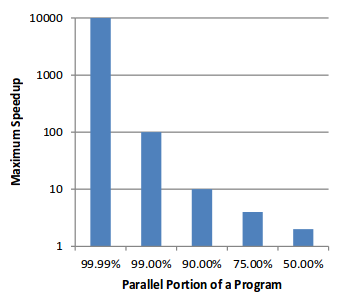
\includegraphics[width=0.5\textwidth]{./Figures/amdahl.png}
  \caption[Amdahl law]{Amdahl law \citep{Reference8}} 
  \label{fig:amdahl} 
\end{figure}

The figures speak for itslelf, to envisage parallel computing, the portion of
parallel code must be very high.

However, Amdahl's law is based on assumption which are hardly verified in
pratique. Following are sumed up reasons not to give to much importance to
Amdahl's law \citep{Reference34}:

\begin{itemize} 
  \item The number of thread is not always always equivalent to the number of processors.  
  \item The parallel portion does not have a perfect speedup. Computation power is used
    for communication between processus. Also some ressources like caches and bandwidth
    have to be shared across all the processors.  
  \item Allocating, delocating and switching threads introduce overhead, overhead growing
    linearly with the number of thread.  
  \item Even an optimized code will not have perfectly synchronised threads, at some point
    some processus will have to wait for others to finish.	
\end{itemize}


Amdahl's law has long been used as an argument against massively parallel
processing. In 1988 Gustafson law came as an alternative to Amdahl's law to
estimate the speedup. In both law, the sequential portion of the problem is
supposed to stay constant. But in Gustafson's law the overall problem size
grows proportionally to the number of cores. As a result, Gustafson's gives
slightly different results to Amdahl's and encourage the use of parallel
computing.\\

However later studies tends to contest the legimity of both laws. Yuan Shi's
paper \citep{Reference9} even proves both theory are but two different
interpretations of the same law. He concludes his study by saying these laws
are too minimalist and what computer scientist really need is a practical
engineering tool that can help the community to identify performance critical
factors.\\

\textbf{Infrastructure implementation}

Beside coding complication, scaling out also brings infrastructure changes.
A third party must be in command of all servers. This master server is also called
load balancer. Its role is to distribute the work evenly between the workers and thus
completly hides the complexity to the user.\\


 % literrature review

\chapter{Experiment}
\label{Chapter3}
\lhead{Chapter 3. \emph{Experiment}}

\section{Client side}



 % Experimental Setup

%\chapter{Experiment} 
\label{Chapter4} 
\lhead{Chapter 4. \emph{Experiment}} 

\section{Client throughout}

\subsection{Client scalability}

SocketCluster-client makes the instanciation of a WebSocket clients on one core
quite straightforward. To deploy it on all available nodes, node.js
\texttt{fork()} function is used. A client code example is given in appendix
\ref{fig:WS_client_simplePing}.

The first experiment is a safety test. It checks if \texttt{fork()} distributes
evenly the work among the cores.

\begin{center}
  \begin{tabular}{ | l | l |}
  \hline
  \multicolumn{2}{|c|}{Parameters} \\
  \hline
    Instance type &  amazon s3 m3.2xlarge\\ 
    Experiment time & 120 s \\
    Number of new communication created at each iteration & 15 \\
    Client creation period & 1 s \\
    Type of ping & random number \\ 
    Ping period & 2.5 s \\ 
  \hline
  \end{tabular}
\end{center}

\begin{figure}[H]
	\centering
		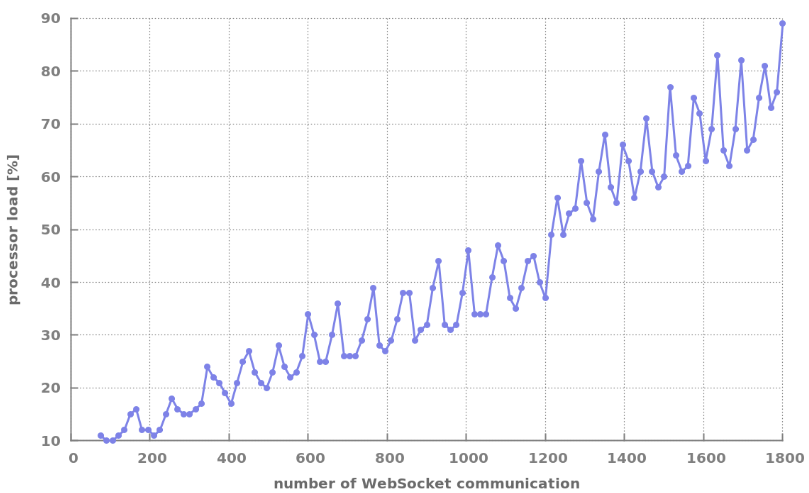
\includegraphics[width=\textwidth]{./Figures/1_client.png}
		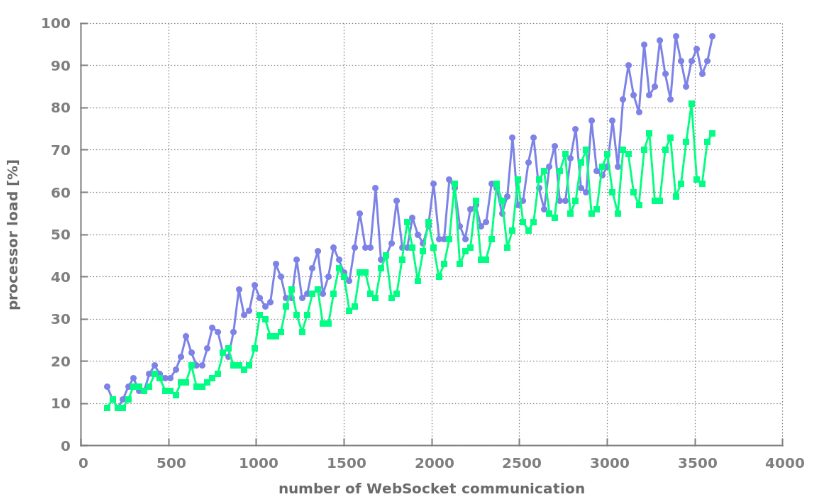
\includegraphics[width=\textwidth]{./Figures/2_client.png}
	\caption[Client throughout]{Client throughout}
	\label{fig:1+2_client}
\end{figure}


From figure \ref{fig:1+2_client} can be inferred that the client
implementation works flawlessly. Adding a second core enables twice as much
communication  to be established.

\subsection{browser testing}

As mentionned in appendix \ref{fig:index_script}, by opering minor changes in
the \texttt{index.html} file, the browser can be configured to display in real
time the number of pings received by a particular worker. If the experiment is
running locally, typing \texttt{localhost:8080} in the url will link the
browser to one worker.\\

\begin{figure}[H]
	\centering
		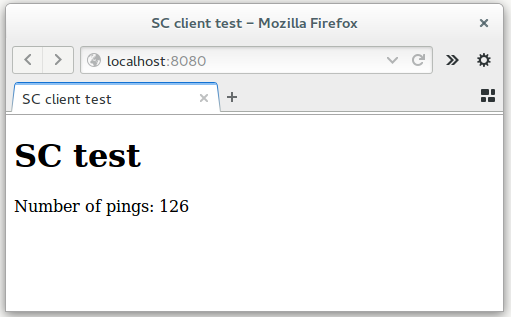
\includegraphics[width=0.9\textwidth]{./Figures/browser.png}
	\caption[Browser connection to SocketCluster]{Browser connection to SocketCluster}
	\label{fig:browser}
\end{figure}

By doing so we can embody a user connected to our WebSocket server and have a
better idea of the reactivity of the server.

% --------------
% second section
% --------------

\section{Comparaison with engine.io}

SocketCluster has been created to ease the creation of multi - core WebSocket
server. Logicaly the first experiment carried out on the server was to compare
a WebSocket to a traditionnal Engine.io server. 

Engine.io and SocketCluster codes can be found in appendix \ref{SocketCluster} and \ref{engine}. 

\begin{center}
  \begin{tabular}{ | l | l |}
  \hline
  \multicolumn{2}{|c|}{Parameters} \\
  \hline
    Instance type &  amazon ec2 m3.2xlarge\\ 
    Experiment time & 60 s \\
    Number of new communication created at each iteration & 20 \\
    Client creation period & 1 s \\
    Type of ping & random number \\ 
    Ping period & 2.5 s \\ 
    Number of clients & 2 \\
  \hline
  \end{tabular}
\end{center}


\begin{figure}[H]
	\centering
		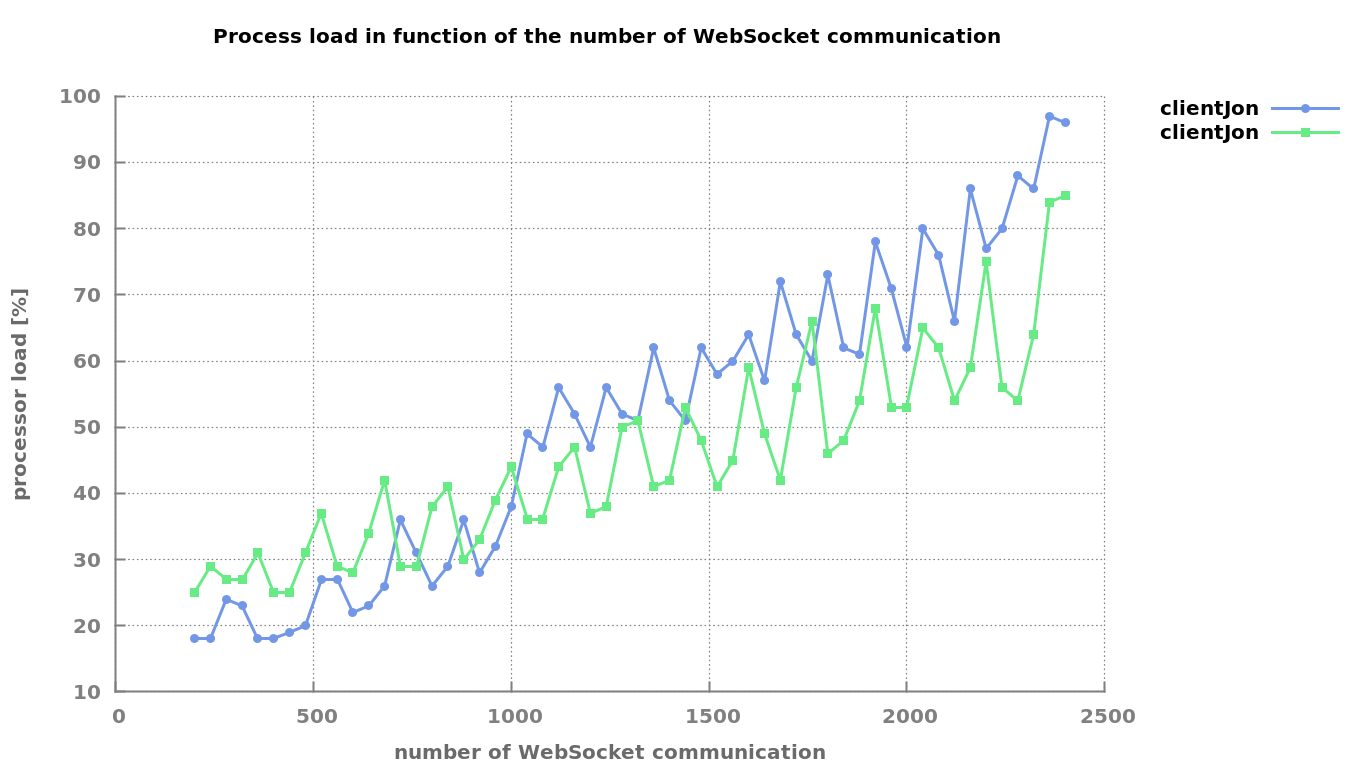
\includegraphics[width=\textwidth]{./Figures/WS_client_comparaison.png}
		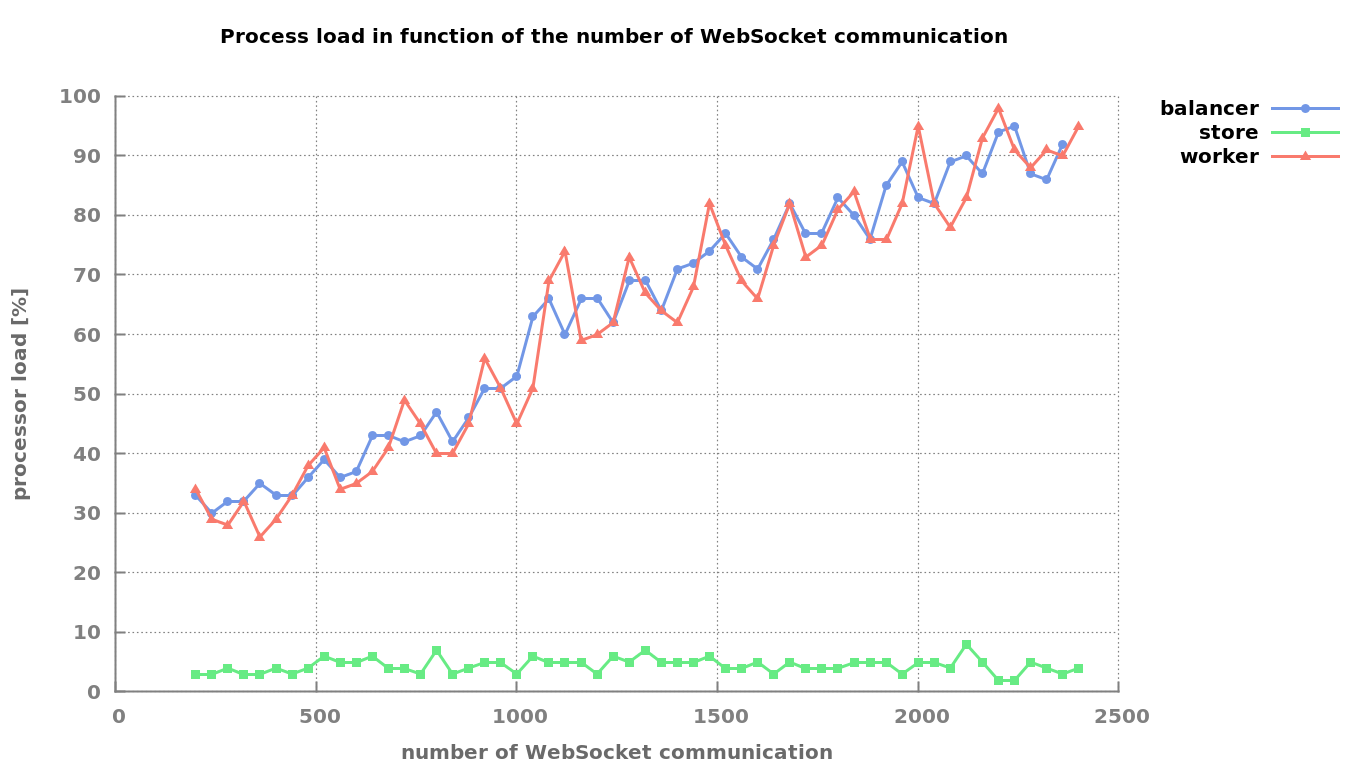
\includegraphics[width=\textwidth]{./Figures/WS_server_comparaison.png}
	\caption[WebSocket implementation]{WebSocket implementation}
	\label{fig:WS_comparaison}
\end{figure}

In this experience, two clients are used to achieve a maximum of 2400 WebSocket
communications.  The server was configured to use one storage, one load
balancer and one worker. While the store processor is quite idle, the two other
processors on the other hand are almost used at full capacity.

\begin{figure}[H]
	\centering
		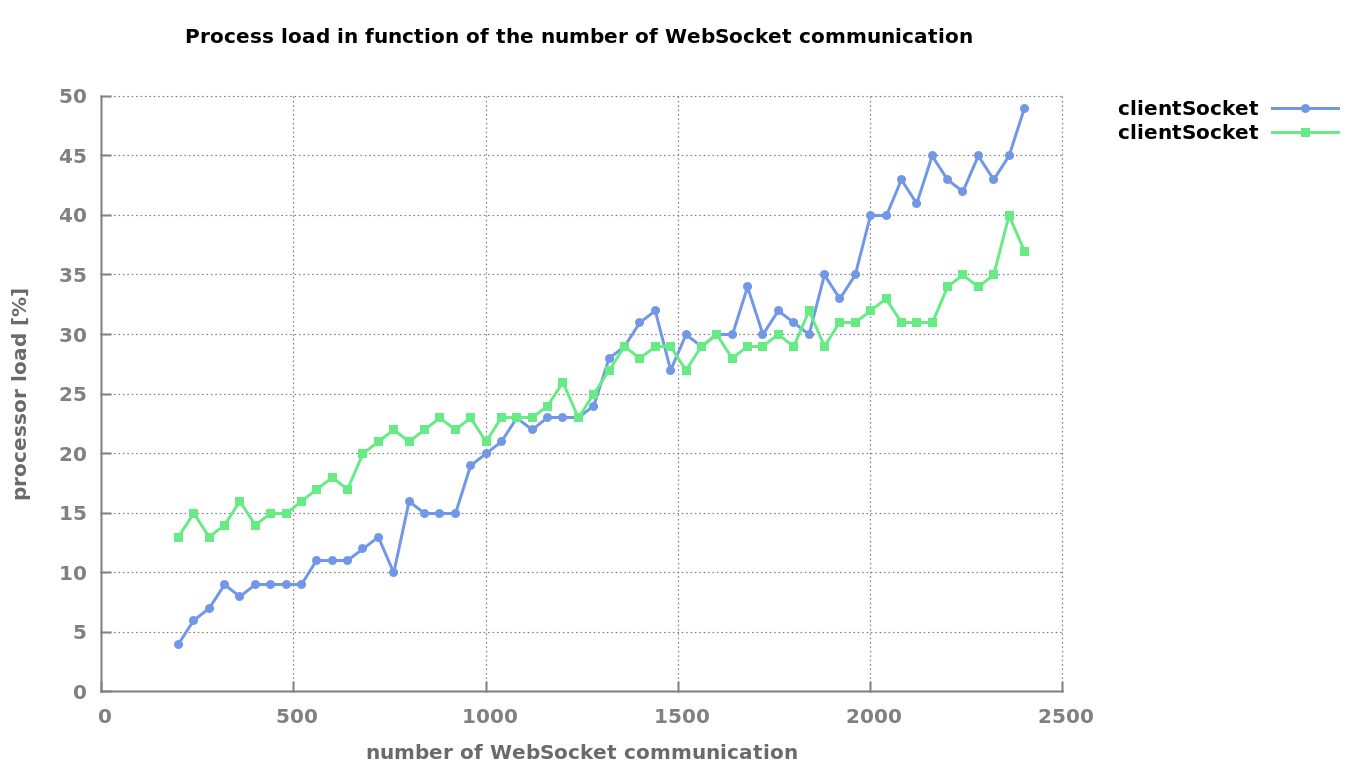
\includegraphics[width=\textwidth]{./Figures/engine_client_comparaison.png}
		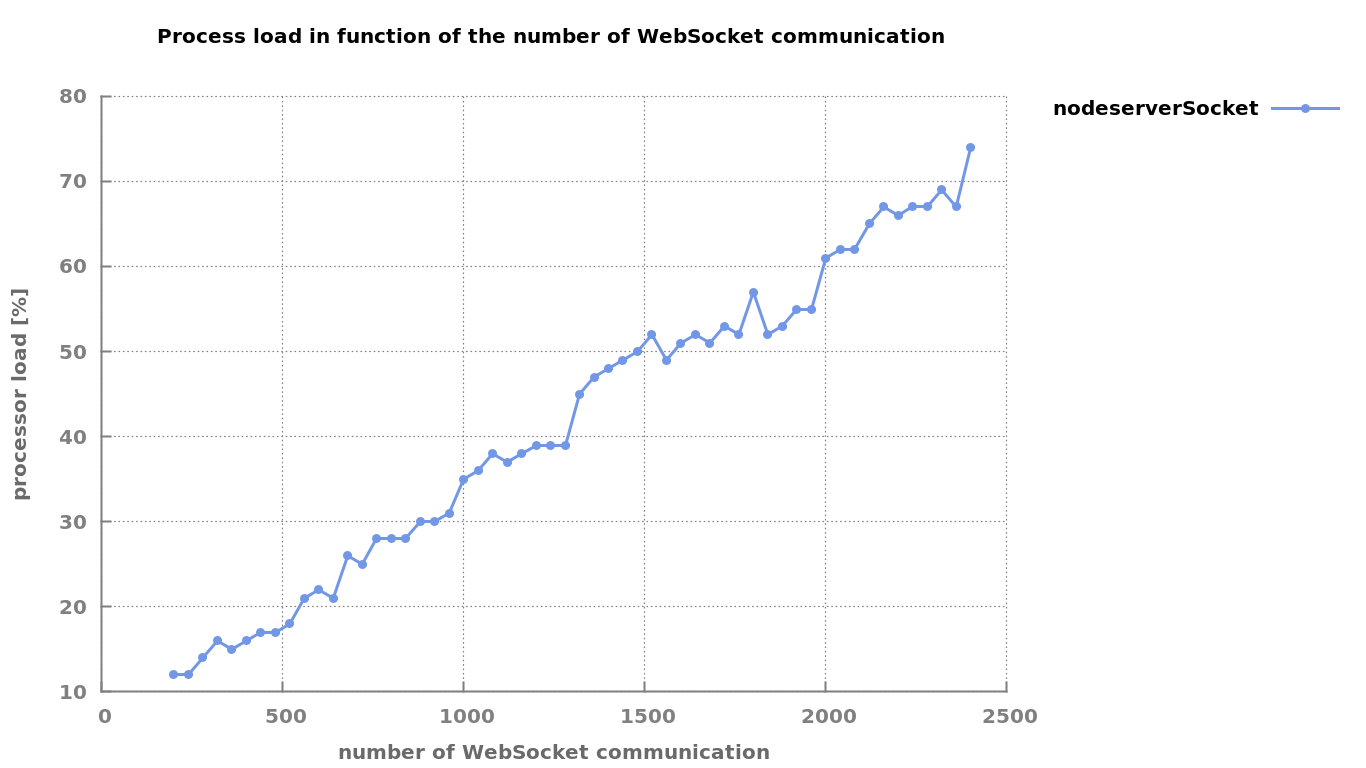
\includegraphics[width=\textwidth]{./Figures/engine_server_comparaison.png}
	\caption[Engine.io implementation]{Engine.io implementation}
	\label{fig:engine_comparaison}
\end{figure}

Surprisingly, pure engine.io implementation seems to be more efficient. Clients
are hitting a maximum of 50\% processor usage compared to 90\% for WebSockets.

On the server side also, engine.io processor peaks at 75\% compared to almost
100\% for WebSockets. Also even if both code have been deployed on similar
virtual machines: \texttt{amazon ec2 m3.2xlarge} the engine.io server is
running only only on one core compared to three for SocketCluster (one storage,
one load balancer and one worker). This seems to show, SocketCluster is not
adapted to low number of communication.

An interesting experiment worth doing at this point, is to try to use
SocketCluster on one core.

% -------------
% Third section
% -------------

\section{SocketCluster context switching}

For this experiment a single core  virtual machine is used for the server:
\texttt{amazon ec2 m3.medium}.

\begin{center}
  \begin{tabular}{ | l | l |}
  \hline
  \multicolumn{2}{|c|}{Parameters} \\
  \hline
    Server instance type &  amazon ec2 m3.medium\\ 
    Client instance type &  amazon ec2 m3.2xlarge\\
    Experiment time & 80 s \\
    Number of new communication created at each iteration & 40 \\
    Client creation period & 1 s \\
    Type of ping & random number \\ 
    Ping period & 2.5 s \\ 
    Number of clients & 2 \\
  \hline
  \end{tabular}
\end{center}

\begin{figure}[H]
	\centering
		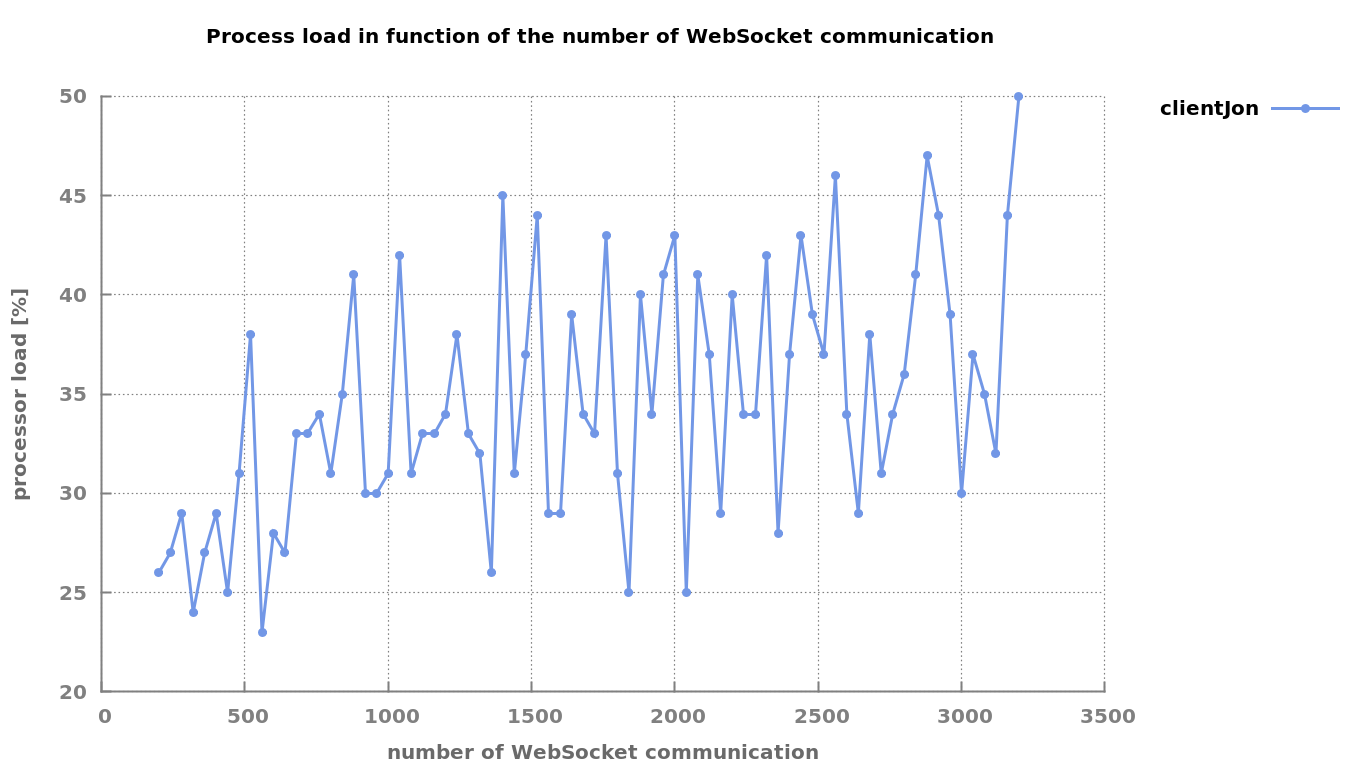
\includegraphics[width=\textwidth]{./Figures/WS_client_context.png}
		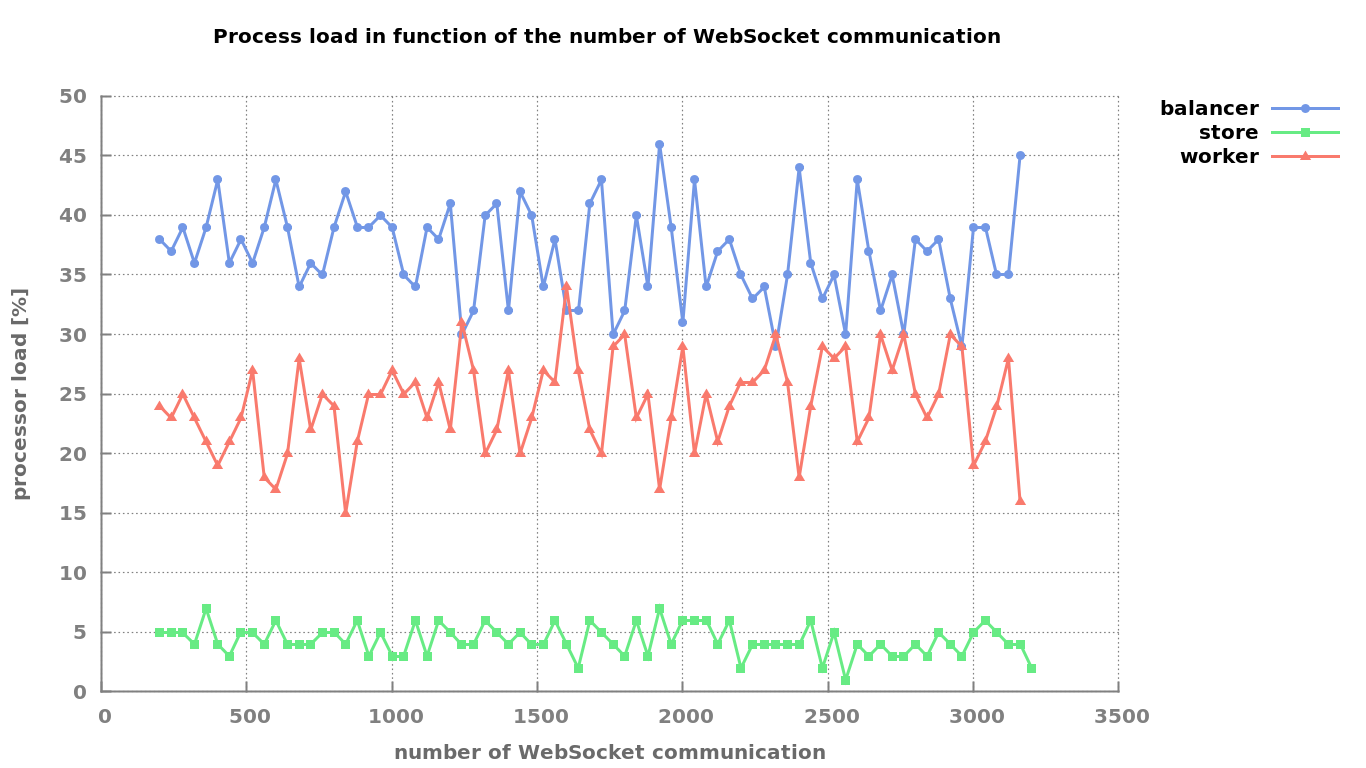
\includegraphics[width=\textwidth]{./Figures/WS_server_context.png}
	\caption[Contexting switching]{Context switching}
	\label{fig:context}
\end{figure}

At the first glimpse, anyone can immediately tell there is a problem with the server
graph. The Load seems to vary randomly at an average of 40\%. What really happens, is
that most WebSocket connections are dropped shortly after beeing created or they 
not even created. The problem is a single core needs to handle four threads. So each
time another application is called the context changes. The result is even worse case of 
a multi-procesor server, because threads then are balanced between processor. Threads 
are heavy weight units, moving them introduces consequent overheads.\\

to conclude, this experiment prooves SocketCluster is not aimed to be used with
project which imvolve more threads than available cores.\\

% --------------
% Fourth section
% --------------

\section{}


\textbf{Client code}

The client code used in all this part is the same. Two clients are used to
produce a maximum of 2400 WebSocket communications.


\begin{center}
  \begin{tabular}{ | l | l |}
  \hline
  \multicolumn{2}{|c|}{Parameters} \\
  \hline
    Instance type &  amazon ec2 m3.2xlarge\\ 
    Experiment time & 60 s \\
    Number of new communication created at each iteration & 20 \\
    Client creation period & 1 s \\
    Type of ping & random number \\ 
    Ping period & 2.5 s \\ 
    Number of clients & 2 \\
  \hline
  \end{tabular}
\end{center}


\begin{figure}[H]
	\centering
		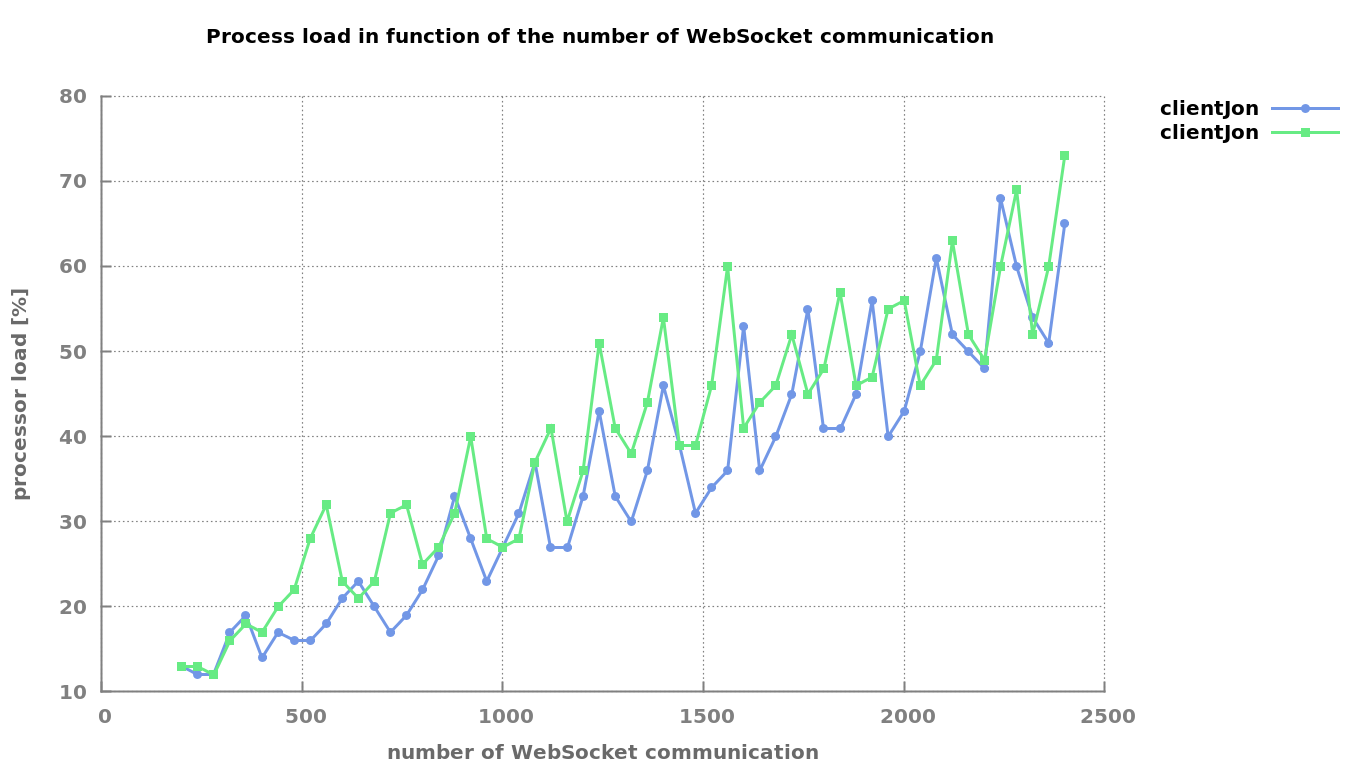
\includegraphics[width=\textwidth]{./Figures/WS_client_rising.png}
	\caption[Simple WebSocket client]{client code}
	\label{fig:WS_client_rising}
\end{figure}

\textbf{Server code}

The first test is run a server using a one store, one load balancer and one
worker.

\begin{figure}[H]
	\centering
		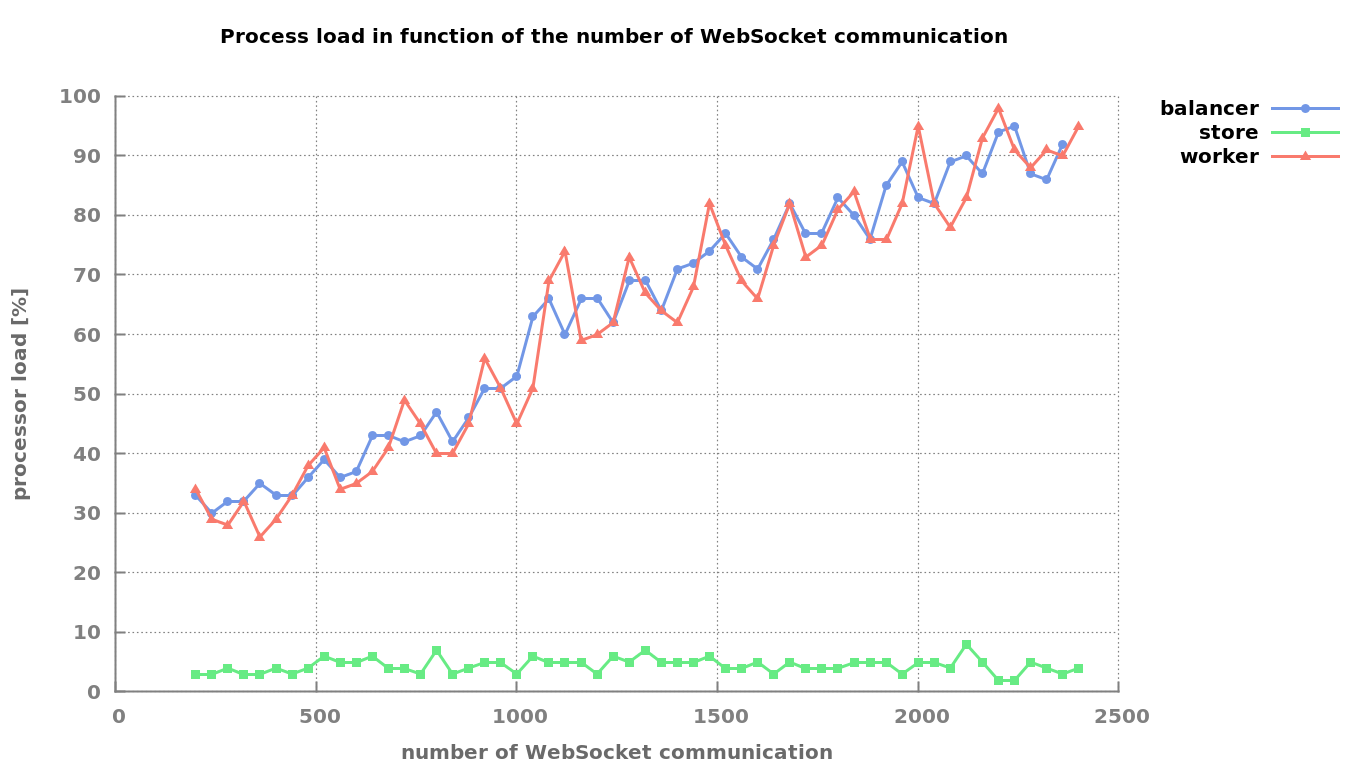
\includegraphics[width=\textwidth]{./Figures/WS_server_1rising.png}
	\caption[WebSocket server on three cores]{Server with 3 cores}
	\label{fig:WS_server_1rising}
\end{figure}

figure \ref{fig:WS_server_1rising} clearly shows the worker and loadbalancer
cores are almost used to their full extent. In order to handle more communication more
cores should be added. 

\begin{figure}[H]
	\centering
		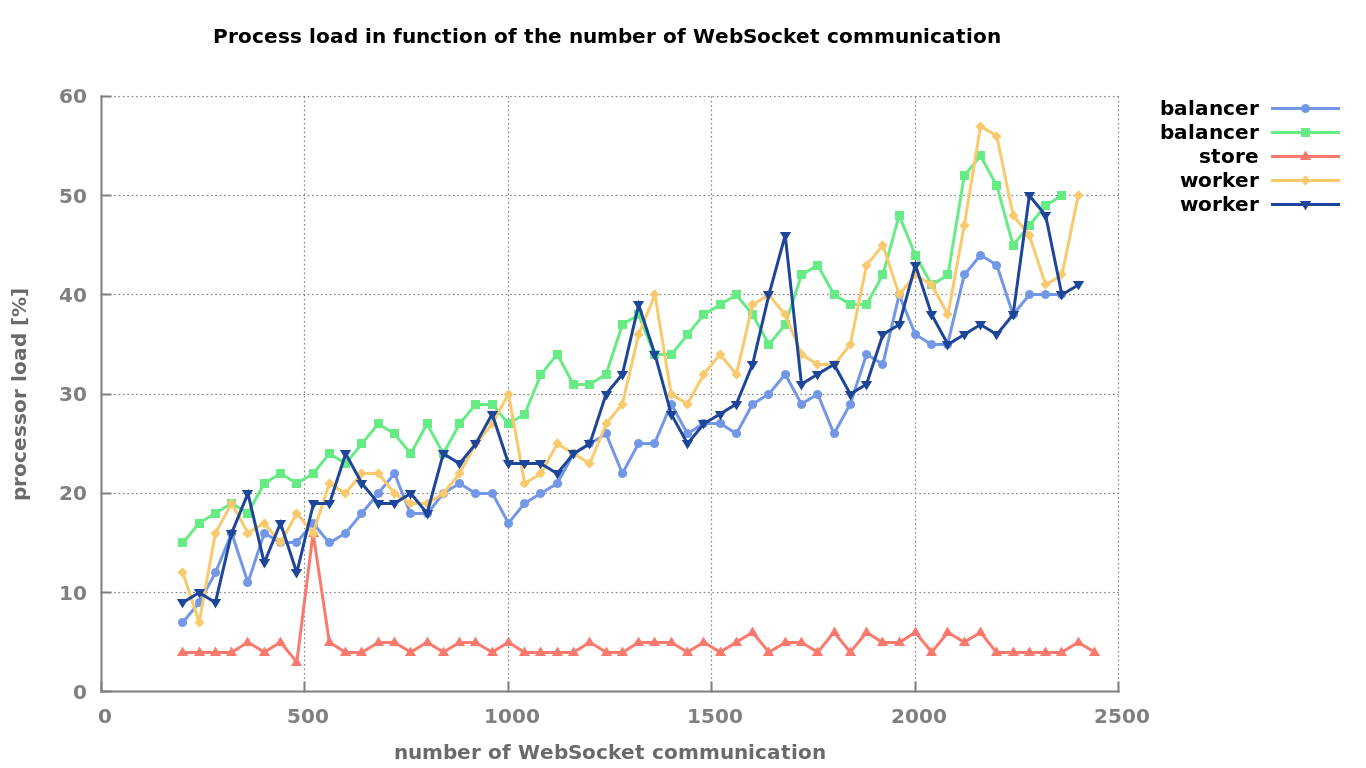
\includegraphics[width=\textwidth]{./Figures/WS_server_2rising.png}
	\caption[WebSocket server on five cores]{server with 5 cores}
	\label{fig:WS_server_2rising}
\end{figure}

In this experiment two more cores have been thrown to work. Load balancers and
workers nicely balance the work between themselves and the maximum load drops to 50\%.

\begin{figure}[H]
	\centering
		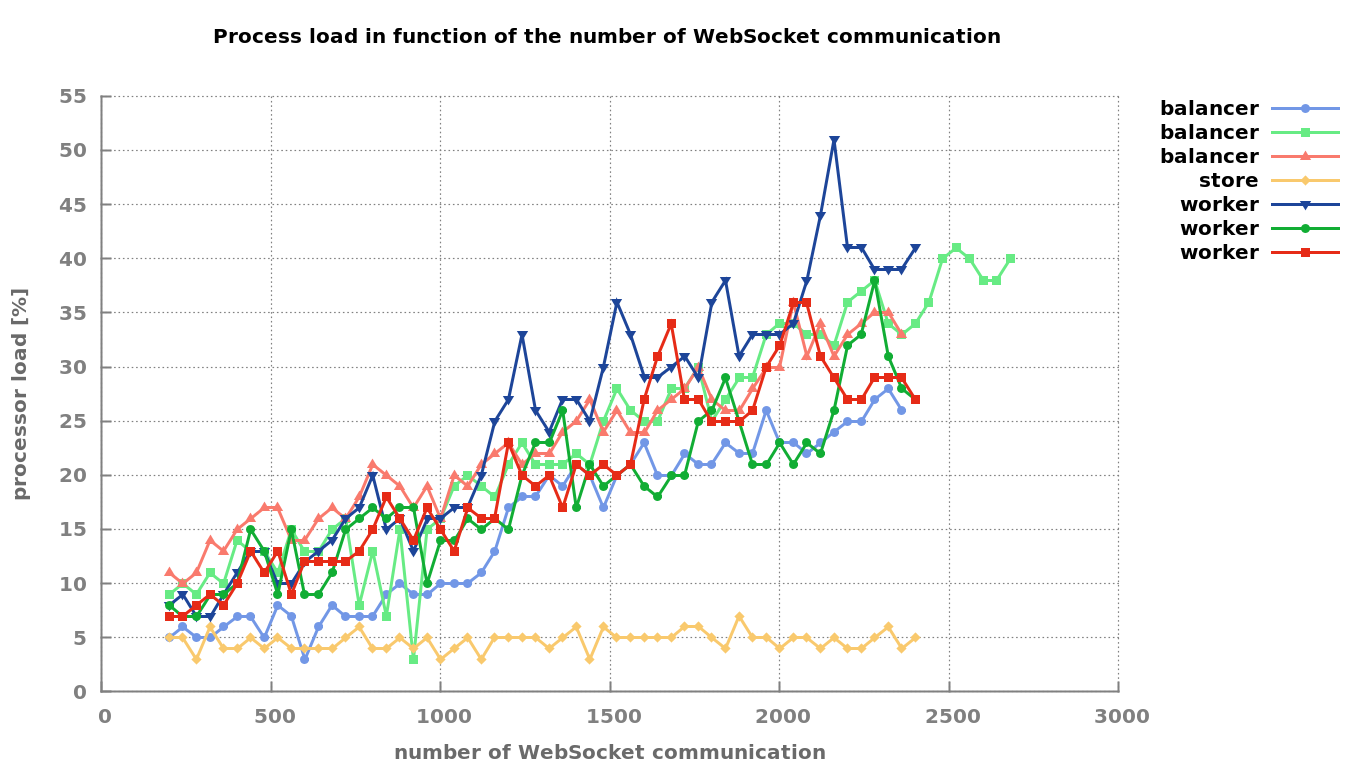
\includegraphics[width=\textwidth]{./Figures/WS_server_3rising.png}
	\caption[WebSocket server on seven cores]{server with 7 cores}
	\label{fig:WS_server_3rising}
\end{figure}

this last test is less conclusive. With a total of 3 cores for load balancers
and three for workers the processors load varies between 30\% and 50\%
depending on the task.\\

Adding too many cores is a waste of ressources, this stresses the importance of
finding a load balancer/worker/store ratio rule.


B] section most influence frequence pings / size message / number communications

c] General rule

load balancer / store / worker
 % Experiment 1

%\chapter{Conclusion} 
\label{Chapter5} 
\lhead{Chapter 5. \emph{Conclusion}} 

After studying the current landscape of research around WebSocket 
in a ditributed environment, this thesis focuses on the benchmarking 
of the node.js's real time engine SocketCluster.\\

SocketCluster is a promising library still actively under development.
It efficiently provides a highly scalable WebSocket server that make
use of all available CPU cores on an instance. It removes the limitation
of having to run Node.js code on single cores.\\

Experiments carried out on SocketCluster revealed two main limitations.  If
running on comparable hardware, a SocketCluster worker will be less efficient
then a basic engine.io implementation. Also SocketCluster efficiency
dramatically drops if run with more process then available cores because of
context switching.\\

Anyway, SocketCluster should be used in highly parallel environment and
therefore these limitations rarely appply. SocketCluster theoriticaly  enables
user to scale an application vertically  without limits. N being the number of
cores the server has, SocketCluster has been prooved to be at least
$\frac{N}{2}$ more efficient then a basic node.js implementation.  As the
number of cores rises, it looks like the performance could be slightly better
then $\frac{N}{2}$. The load balancers begins to missbehave and performances
are limitted by a few overloaded load balancers. However, it is probably only a
question of time until a patch fixes this issue.\\

While benchmarking SocketCluster, useful SocketCluster features were
considered.  System administrator could benefit from a realtime monitoring tool
to check the state of each threads and thus help them manage the size of the
cluster. The monitoring tool could even be linked with an algorithm to
automatically append or delete threads.  SocketCluster would then be an autonom
entity. Scaling on its own without any human interaction.\\



 % Experiment 2

%\input{./Chapters/Chapter6} % Results and Discussion

%\input{./Chapters/Chapter7} % Conclusion

%% ----------------------------------------------------------------
% Now begin the Appendices, including them as separate files

\addtocontents{toc}{\vspace{2em}} % Add a gap in the Contents, for aesthetics

\appendix % Cue to tell LaTeX that the following 'chapters' are Appendices

\chapter{SocketCluster}
\label{SocketCluster}
% \lhead{Appendix A. \emph{SocketCluster}}
\section{Simple ping-pong exchange}
\textbf{Client code}


This is an example of a WebSocket client code spread on all available cores.
New clients are spawned every \texttt{numberClientsEachSecond}. Thereafter,
every \texttt{intv} each clients sends a ping event cast to a Javascript JSON
object.

\begin{figure}[H]
	\centering
		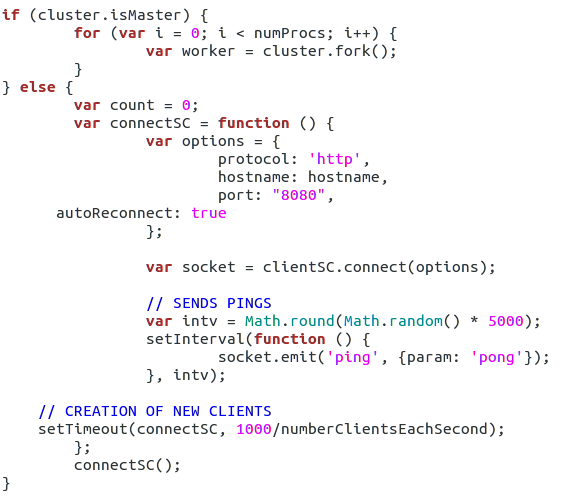
\includegraphics[width=0.7\textwidth]{./Figures/WS_client_simplePing.png}
	\caption[WS_client_simplePing]{Pings from client}
	\label{fig:WS_client_simplePing}
\end{figure}

To best simulate clients interaction with a websocket server, new sockets are
created at random intervals \texttt{intv = Math.round(Math.random()*5000)}.

\textbf{Server code}

The server listens for pings event and answers back with pongs event. In this
case the pong event is an integer counting the number of pings this particular
worker had during the whole experiment.

\begin{figure}[H]
	\centering
    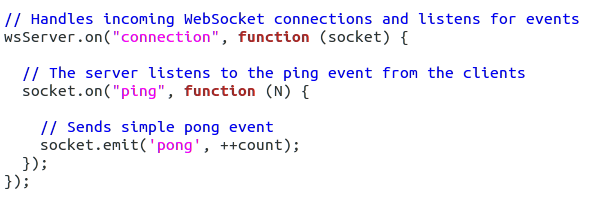
\includegraphics[width=0.9\textwidth]{./Figures/WS_server_simplePong.png}
	\caption[WS_server_simplePong]{Server answering with pongs}
	\label{fig:WS_server_simplePong}
\end{figure}

\section{File transfer}

\textbf{Client code}

In this example, the goal is to exchange a file using the WebSocket protocol.
For this purpose, the node.js \texttt{delivery} library is used.

New clients are created on the same model as the previous exmample. Each new
client is stored in the \texttt{clients} array. Each clients are also
perdiodically sending pings. The only add on is the \texttt{map} function to
enable the each socket to retrieve the document sent by the server. 

\begin{figure}[H] \centering
  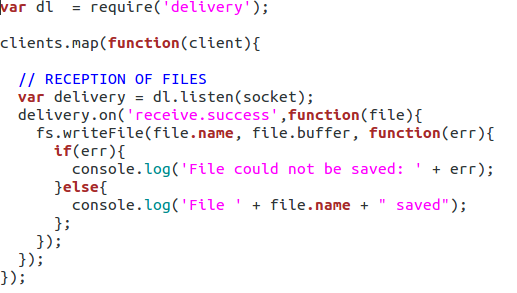
\includegraphics[width=0.9\textwidth]{./Figures/WS_client_delivery.png}
\caption[WS_client_fileTransfer]{Clients receptionning files} 
\label{fig:WS_client_fileTransfer}
\end{figure}

\textbf{Server code}

The server listens for pings. And sends back a file, \texttt{foo.txt} in this
example.

\begin{figure}[H]
	\centering
    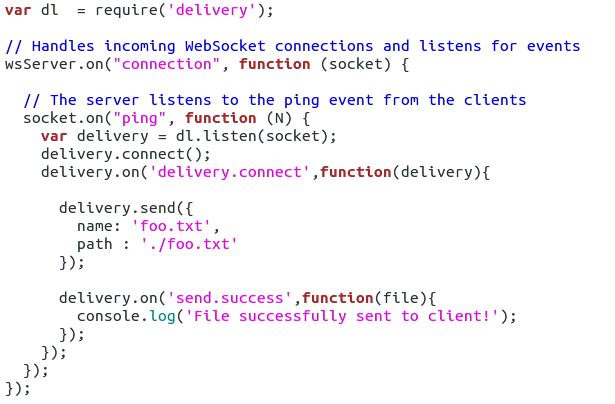
\includegraphics[width=0.9\textwidth]{./Figures/WS_server_delivery.png}
	\caption[WS_server_simplePong]{Server sending files}
	\label{fig:WS_server_simplePong}
\end{figure}
	% Appendix Title

%\chapter{Engine.io}
\label{engine}
% \lhead{Appendix A. \emph{SocketCluster}}

This appendix gives the code used to create a simple engine.io server and
client. Comparaison with SocketCluster code in appendix \ref{SocketCluster} 
shows the difference between both implementation is small. 

In fairness, SocketCluster API is very close to engine.io.

\textbf{Client code}

\begin{figure}[H]
	\centering
		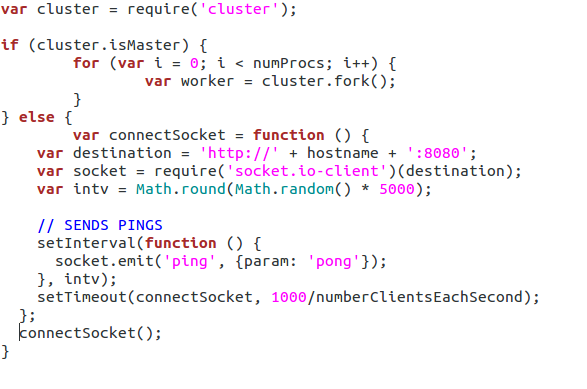
\includegraphics[width=0.9\textwidth]{./Figures/engine_client_simplePong.png}
	\caption[Engine.io client code]{Pings from client}
	\label{fig:engine_client_simplePing}
\end{figure}


\textbf{Server code}


\begin{figure}[H]
	\centering
    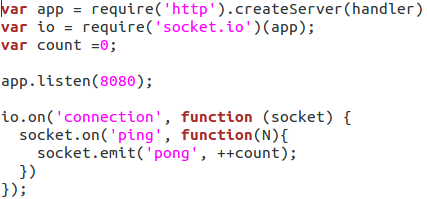
\includegraphics[width=0.7\textwidth]{./Figures/engine_server_simplePing.png}
	\caption[Engine.io server code]{Server answering with pongs}
	\label{fig:engine_server_simplePong}
\end{figure}

 % Appendix Title

%\chapter{Real time throughout check}
\label{indexHTML}

By inserting the following script in \texttt{index.html} the browser will
display in realtime the number of pings received by a WebSocket server.

\begin{figure}[H] \centering
  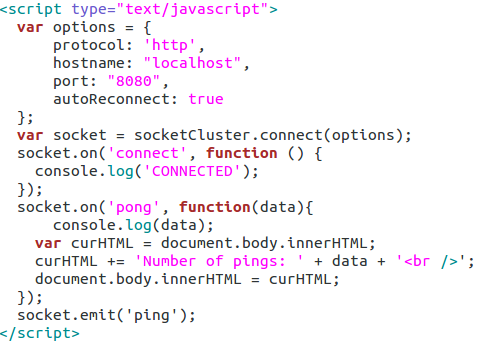
\includegraphics[width=0.8\textwidth]{./Figures/index_script.png}
\caption[index_script]{Modification to \texttt{index.html}}
\label{fig:index_script} \end{figure}

All it does is emitting a ping, then listening to the pong event and displaying
it directly in the html page. The pong payload as can be seen in
\ref{fig:WS_server_simplePong} is \texttt{count}, an integer increamented each
new ping.
 % Appendix Title

\addtocontents{toc}{\vspace{2em}}  % Add a gap in the Contents, for aesthetics
\backmatter

%% ----------------------------------------------------------------
\label{Bibliography}
\lhead{\emph{Bibliography}}  % Change the left side page header to "Bibliography"
\bibliographystyle{unsrtnat}  % Use the "unsrtnat" BibTeX style for formatting the Bibliography
\bibliography{Bibliography}  % The references (bibliography) information are stored in the file named "Bibliography.bib"

\end{document}  % The End
%% ----------------------------------------------------------------
